\graphicspath{{images/methodology/}}
\section{Reinforcement learning method}
The reinforcement learning method trains an agent to take the optimal sequence of decisions \cite{sutton2018reinforcement}. The learning process uses positive and negative reinforcement to increase or decrease the probability of choosing an specific action. In this sense, the agent learns, through an iterative process, to make the sequence of decisions that maximizes the amount of reward that he will receive \cite{sutton2018reinforcement}.

\begin{figure}[h!]
	\centering
	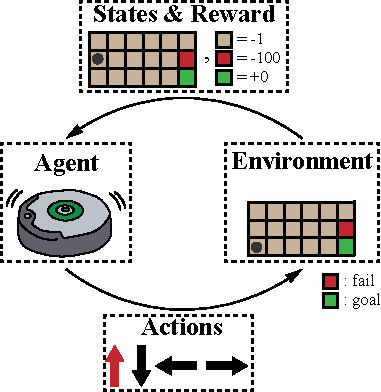
\includegraphics{reinforcement_learning_diagram.pdf}
	\caption{Reinforced learning framework for the application that a mobile robot must reach the desired position. In this example, the agent's actions are up, down, right and left; likewise, the agent's objective is reach the green cell and the agent fails when reach the red cell.}
	\label{fig:RL_framework}
\end{figure}

The framework of reinforcement learning is formed by four elements: (i) agent, (ii) actions, (iii) environment, and (iv) states and rewards \cite{sutton2018reinforcement}. Figure \ref{fig:RL_framework} describes the reinforcement learning framework for the application that a mobile robot must reach the desired position. First, an agent is the entity who takes decisions based on the reward and punishment that he will receive. Second, action space are all the available actions that the agent could use to interact with the environment. Third, the environment is the space where the agent lives and interact. Fourth,  the new agent's state after applying an action in the environment and the reward associated with that specific action. This process will be repeated several times until the agent learns a successful strategy to interact with the environment and maximize the reward.

In reinforcement learning, the agent's strategy is called policy ($\pi(s|a)$) and indicates which actions the agent should chooses in each state \cite{sutton2018reinforcement}. Policies are usually stochastic to consider the uncertainties and probabilities of real world \cite{tedrake2004stochastic}.  In this way, policies assign a probability of success to each action, and the agent chooses the action with the highest probability. Hence, the objective of reinforcement learning algorithms is to find the optimal policy that maximizes the amount of reward. 

The sum of the accumulated rewards from an initial state $s_t$ is the standard way of quantifying how good or bad the policy is \cite{sutton2018reinforcement}. This quality parameter is called value function ($V^{\pi}(s_t)$) and indicates the discounted sum of rewards that an agent will obtain starting in state $s_t$ and following the policy $\pi$ \cite{sutton2018reinforcement}. The value function can be computed as
\begin{equation*}
	V^{\pi}(s_t= s) = E_{\pi}  \left[r_t + \gamma r_{t+1} + \gamma^{2} r_{t+2}+ . . . | s_t = s \right],
\end{equation*}
\noindent where $r_t$ is the reward at time $t$, $\gamma$ is a discounted term and $s_t$ is the initial agent's state. However, calculating the value function requires the agent to start in all available states of the environment and in complex activities this can require a large amount of storage and computational cost. For this reason, more recent work uses deep neural networks to estimate the value function and optimal policy \cite{henderson2018deep}.


\begin{figure}[h!]
	\centering
	\subfloat[]{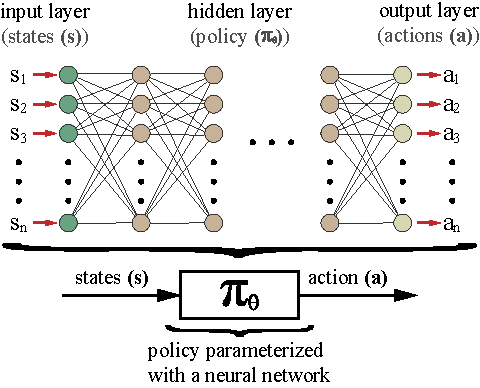
\includegraphics{policy_cnn.pdf}}
	\hfill
	\subfloat[]{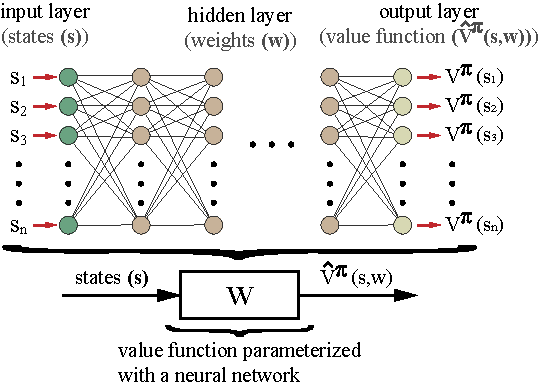
\includegraphics{value_function_cnn.pdf}}
	\caption{Deep neural networks scheme: (a) predict optimal action and (b) estimate value function.}
	\label{fig:rl_cnn}
\end{figure}

\section{Deep reinforcement learning}
Deep reinforcement learning (DRL) represent the combination of deep neural networks with reinforcement learning framework \cite{li2017deep}. Deep neural networks estimate the value function and predict the policy actions considering agent's state as input. Figure \ref{fig:rl_cnn} describes the policy and value function parameterized with a neural network. Therefore, the goal of DRL is to find the neural network parameters that describe the optimal policy that generates the highest reward.

The policy gradient method optimizes the parameters of a neural network that define the behavior of the policy, and in this way, maximize the accumulated reward \cite{sutton2018reinforcement}. The policy gradient algorithms formulate an objective function related to the accumulated reward and then use the gradient ascent method to modify the parameters of the neural network~\cite{thomas2017policy}. A general objective function is given by

\begin{equation*}
	L(\theta) = \expectation \left[ \mathrm{log} \pi_\theta (a|s) \advantage  \right],			
\end{equation*}
with,
\begin{equation*}
	\advantage = V^{\pi_{\theta}}_{t}  - \hat{V}_{t}, 
\end{equation*}
\noindent where $\advantage$ is advantage function, $V^{\pi_{\theta}}_{t}$ is accumulated reward following policy $(\pi_\theta)$ and $\hat{V}_{t}$ is expected accumulated reward by the neural network.


\section{Proximal policy optimization}
PPO is a recent policy gradient method that strikes a good balance between rapid implementation and efficiency \cite{schulman2017proximal}. The objective function of PPO seeks to maximize accumulated reward, minimize estimation error of value function and explore different sequence of actions. For this purpose, 


\begin{equation*}
	L^{\mathrm{PPO}}(\theta) = \expectation \left[  L^{\mathrm{CLIP}}(\theta) - c_1 L^{\mathrm{VF}}(\theta)  + c_2 S[\pi_\theta](s_t)  \right],			
\end{equation*}	
with,
\begin{equation*}
	L^{\mathrm{VF}}(\theta) = \left( V_\theta (s_t) - V^{\mathrm{target}}_{t}  \right)^{2},
\end{equation*}			

\begin{equation*}
	L^{\mathrm{CLIP}}(\theta) = \expectation \left[ \mathrm{min} \left(  r_{t}(\theta)  \advantage,  \mathrm{clip} (r_{t}(\theta) , 1-\epsilon, 1+\epsilon) \advantage  \right)  \right],			
\end{equation*}	



%the development of a bipedal robot controller, made in the simulator for multi-body dynamics MuJoCo, with the use of the deep reinforcement learning algorithms class Proximal Policy Optimization (PPO). In addition, an analysis will be carried out on the joints of the robots to understand the degree of importance of each one of them in the gait learning process.


%based on reward or punish an specific behavior \cite{sutton2018reinforcement}. In this way, the model take decisions/actions and learn through trial and error. The framework is formed by four parts: (i) agent, (ii) action, (iii) environment and (iv) reward. This learning method maintains growing interest in development due to its simplicity and powerful problem-solving capabilities.







\section{Related work}

Currently, there are several methods to develop drivers for robots with legs. The classic ones use previous knowledge about the robot, such as its dynamic model or information obtained from simulations involving them. For example, the ANYmal robot from ETH uses the inverted pendulum model to generate joint torques, contact forces and motion \cite{anymal}; the MIT Cheetah uses a model predictive control to plan desired contact forces \cite{cheetah}.

However, in certain cases, it can be difficult to obtain prior knowledge of the robot through dynamic models and simulations. In this context, a feasible approach to controller design is to use deep learning, more specifically, deep reinforcement learning. Furthermore, another advantage that the use of machine learning provides is that it does not accumulate data generated by the robot, it only uses what is currently being processed, in addition to the fact that the robot can learn to march on its own \cite{haarnoja2018learning}.

Controller development methods using deep reinforcement learning may vary depending on the chosen algorithm. The University of California, for example, used a learning algorithm based on maximum entropy reinforcement learning, training a Minitaur robot directly, without having to train a simulation beforehand \cite{haarnoja2018learning}.

In this work, a class of deep reinforcement learning algorithms — Proximal Policy Optimization (PPO) — will be used to train a simulation of a biped developed in MuJoCo, a simulator for multi-body dynamics.


